\section{Social Weaver Analysis}
\subsection{Social Weaver in Action}
This chapter will lead us through an real example where Social Weaver is being used. It will be explained which components are used in what situations and how they interact with each other. Because we used the Google Calendar example several times it is only fair to use it finally for an overview.

\subsubsection*{Initial Scenario}
The following explanations will be based on a scenario with two users (Alice and Bob) who both are running the Social Weaver plugin in Firefox and are connected to the same Web Service (which means they share the same Social Weaver session). 

Additionally they obviously need a shared google calendar. For accessing the calendar they use the default web service provided by Google and no alternative client. 

The scenario will consists of the following steps:
\begin{enumerate}
	\item Alice weaves a comment box to an appointment in the shared calendar
	\item Alice uses the comment box to leaves a question
	\item Bob logs in and anwers Alice's question
	\item We manually destroy the anchor directly in the database
	\item Alice recognizes this failure and relinks the comment box
\end{enumerate}

In the following two sub-procedures, update and matching, will be explained. The reason why we handle those seperately is, that we will use them more frequently in the whole process. That way we can just refer to them and keep the focus on the actual workflow. 

\subsubsection*{Update Procedure}
The synchronisation for Social Weaver is quite simple. Basically the plugin sends at start up (or when asked) two parameters in a JSON array to the web service using a authenticated POST request. Those parameters are the current URL and the timestamp of the last update. If Alice starts up her first browser the first time, the plugin would send the following JSON file:

% TODO nochmal pruefen

\begin{lstlisting}[language=JavaScript]
{
	last_update=12341234,
	current_url='www.cal.google.com'
}
\end{lstlisting}

The web service uses those information to determine whether there are new and relevant anchors or not. In the positive case (see Figure \ref{sequence-update}) the anchors are returned. In Alice's case nothing will be returned since we have no marked elements. 

What happens at the server with those data in detail? We use the timestamp of the last update and the current URL to create a query that receives only the corresponding anchors. 

Through a simple HTTP header authentication we know which user is getting access to the anchor data. Even though it is not really relevant in our simple case. It would be more an issue when having multiple users in different session in one Social Weaver context. But such scenarios will not be covered in this thesis.

\begin{figure}[h!] \centering
		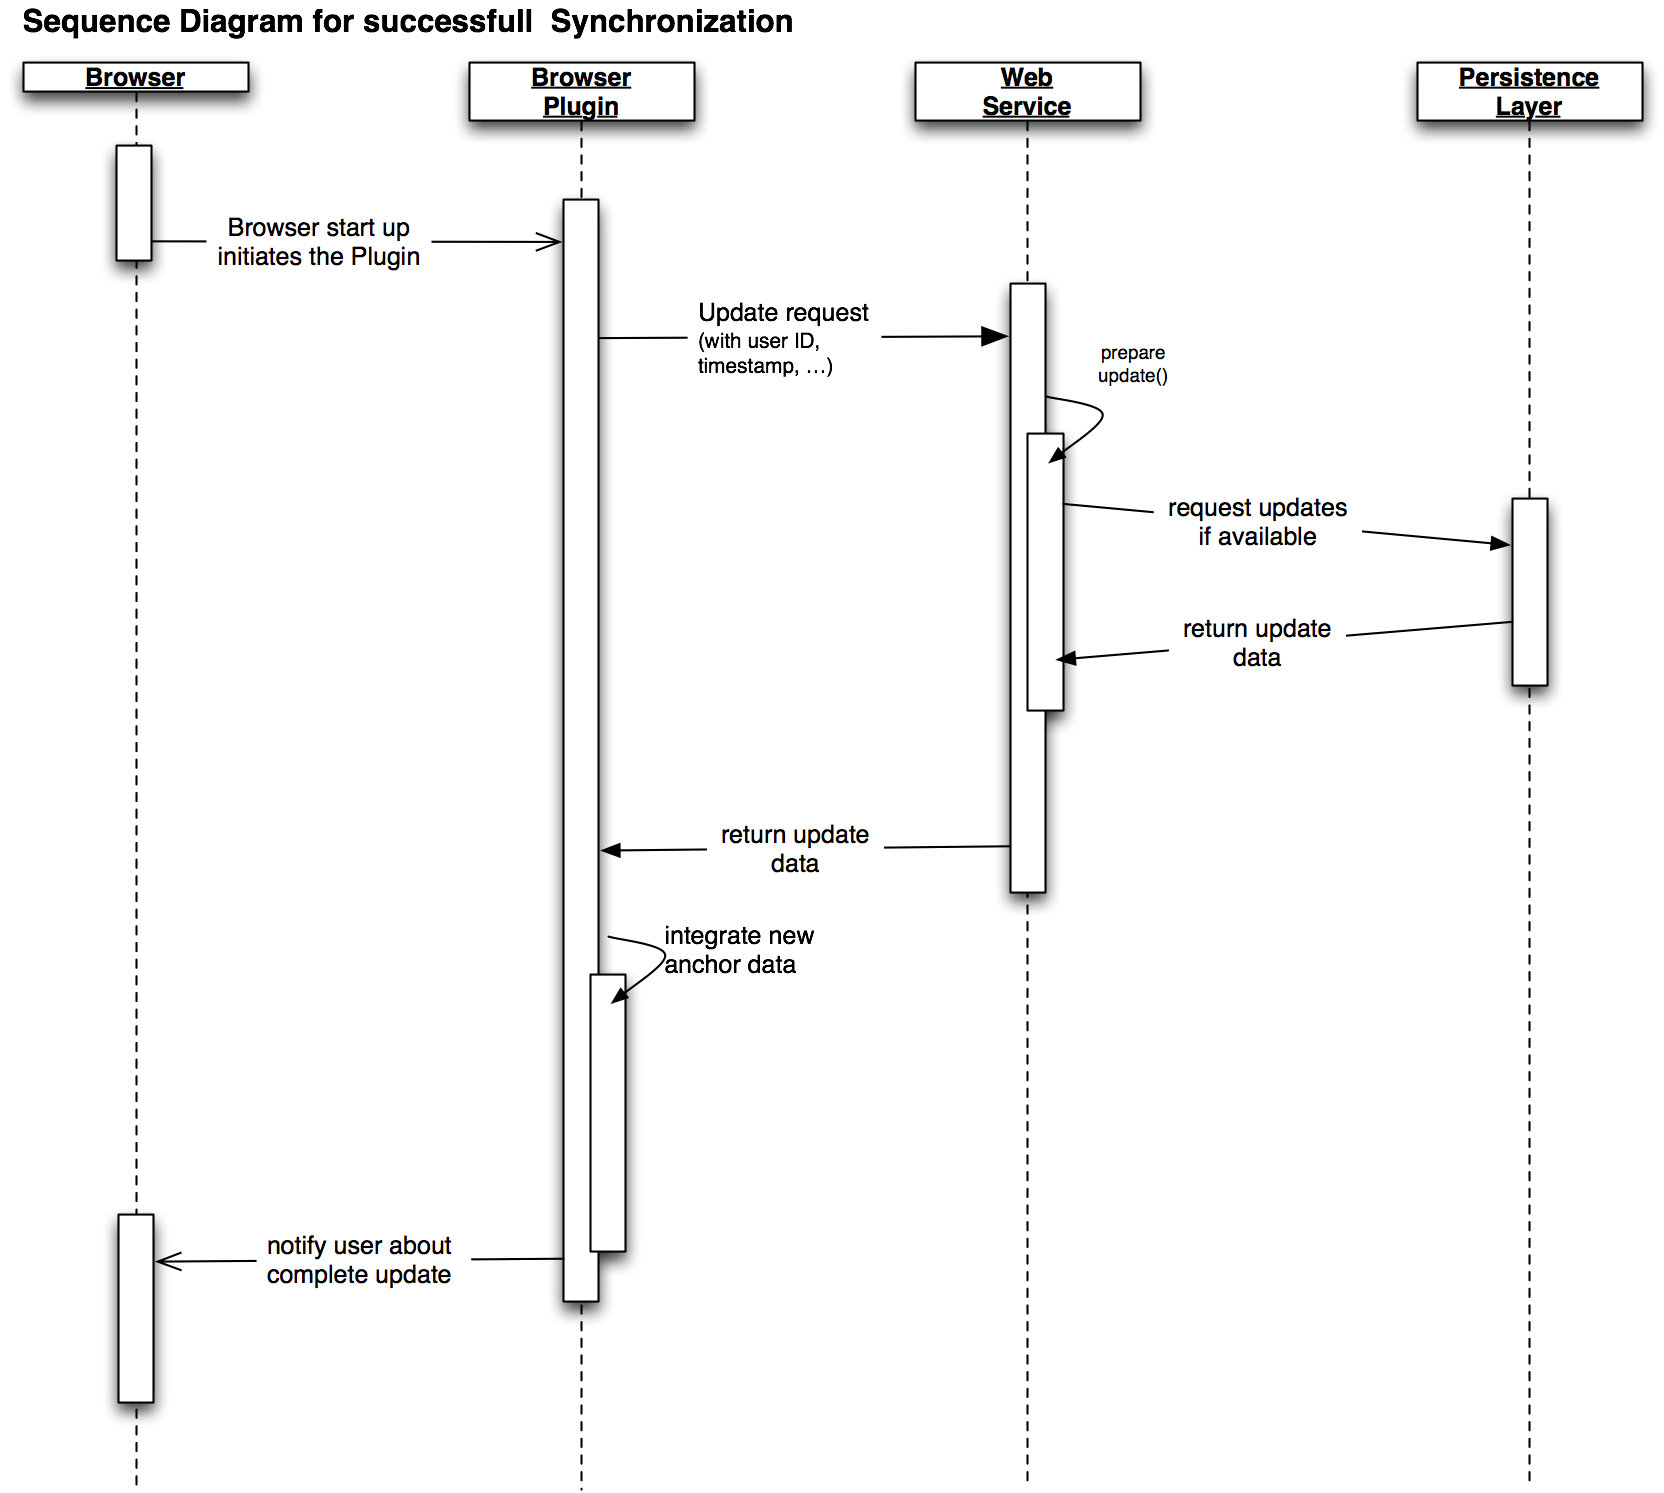
\includegraphics[width=13cm]{images/sequence-update.png}
		\caption{Sequence diagram for a successful plugin update}
		\label{sequence-update}
\end{figure} 

\subsubsection*{Matching Procedure}
When we use the term matching procedure it means that exisiting anchors are visualized to the user. Before every matching procedure we assume that an update is triggered to ensure that the newest data is being used. 

Beyond the update procedure there is no need communicate with the server. When the user opens a new URL it triggers the matching procedure. The plugin searches its local content whether there are some anchors for this URL. In a positive case (see Figure \ref{sequence-matching-process}) the content is visualized to the browser view. 

At this point Alice would recieve nothing from the plugin since no anchors exist for \verb+www.cal.google.com+. 

The way how anchors are retrieved from the plugin is quite similar how it is done at the backend. The major difference is that we do not use any timestamps at this time. There is no need for that since we assume everything is up to date after the update procedure. 

\begin{figure}[h!] \centering
		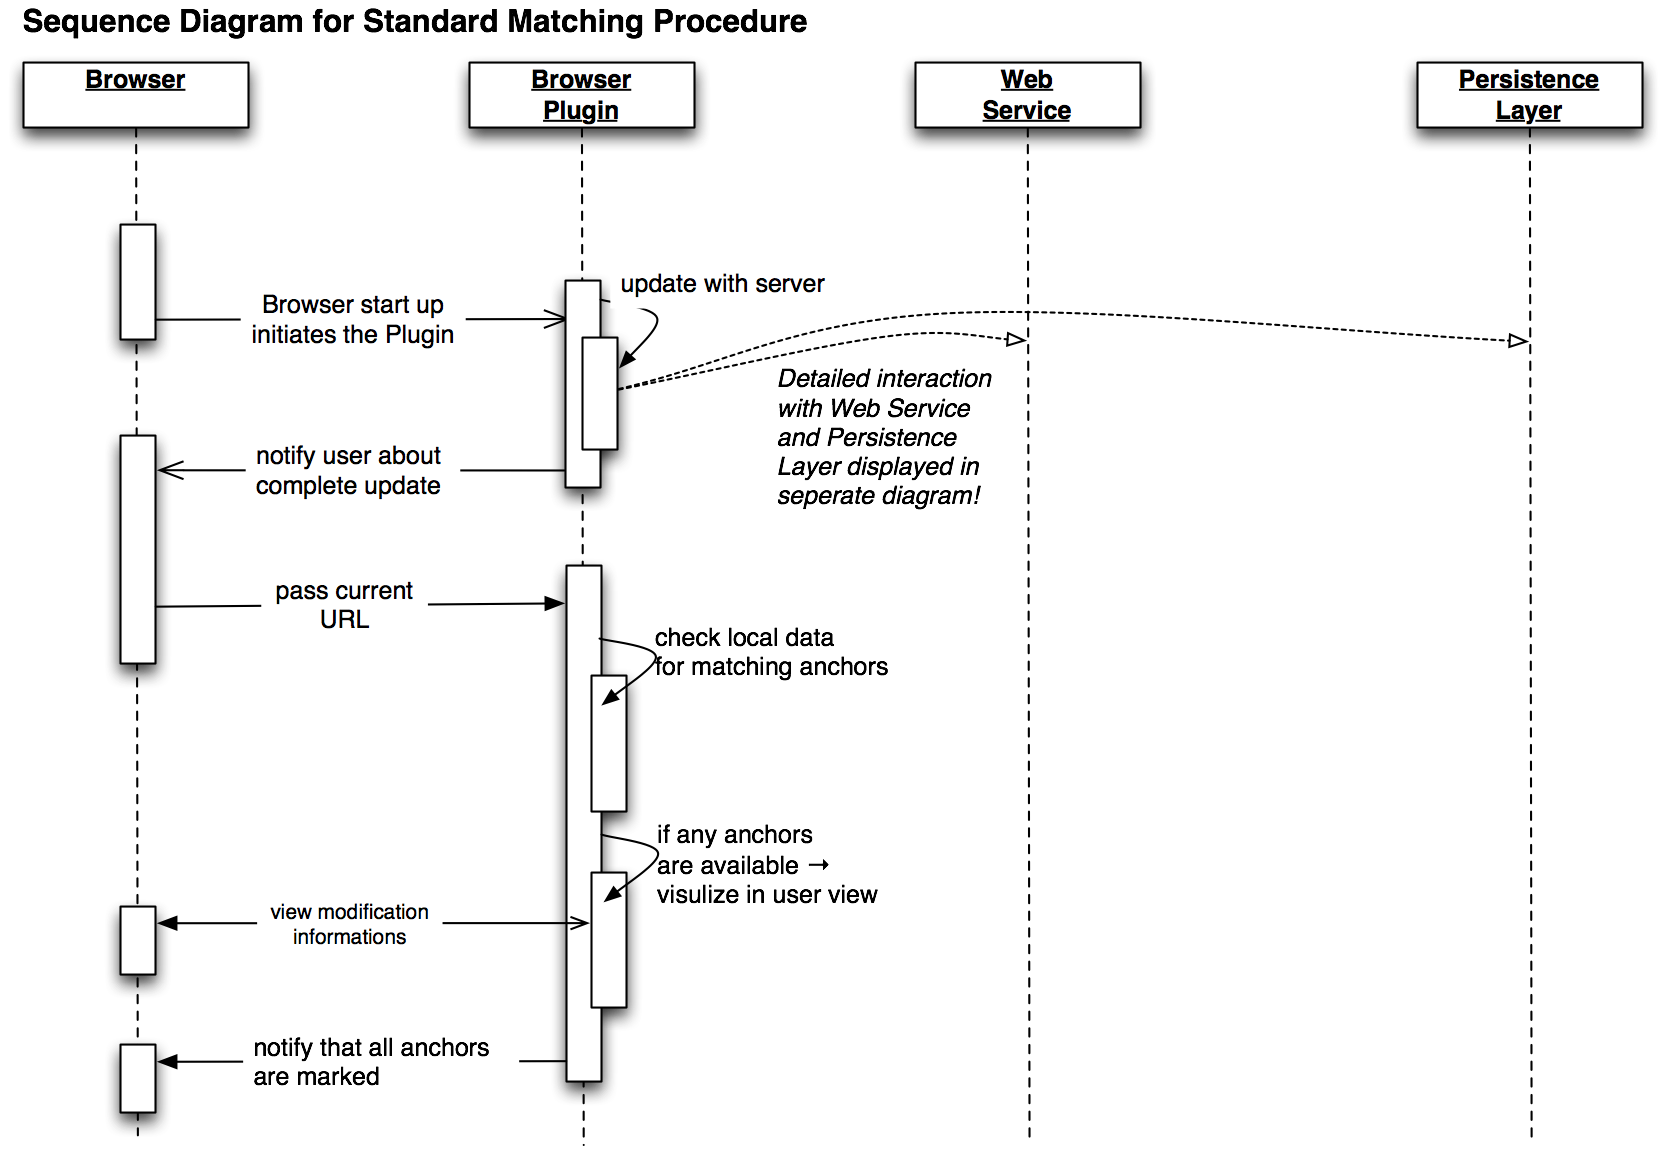
\includegraphics[width=13cm]{images/sequence-matching-process.png}
		\caption{Sequence diagram for a standard matching procedure}
		\label{sequence-matching-process}
\end{figure} 

\subsubsection*{Scenario Execution}
Now that we learned about the two sub-procedures we are able to start with the actual scenario. First step is going to be that Alice weaves a comment box to an appointment: 

Alice enters \verb+www.cal.google.com+ which first of all triggers an update. Afterwards potentially new anchors would be displayed in the browser - which is not the case right now. 
Now Alice is able to mark an appointment. By clicking an element (in edit mode, see ???) she appends a comment box. 
In the background the plugin runs the script (or scripts) that are related to the URL to define an identifier for the element. 
Using this identifier, the content-data for the comment box and the current URL the plugin creates a message in JSON format and passes it to the server. 

The content for the comment box in this case is just a link. We use an external comment system that will be injected as HTML code. Where or how exactly this comment box is defined, is not relevant to our matters.

For our example the JSON file mights look like:

\begin{lstlisting}[language=JavaScript]
{
	content-data='www.chatsystem.com/alice-apointment-17349',
	element-id='7234808234088023480',
	current-url='www.cal.google.com'
}
\end{lstlisting}

The message is passed as an authenticated POST Rest request. The web service performs some checks before the anchor is persisted. For instance it could be the case that there is already an anchor for exactly this element (because an other user created one in the meantime or the element identifier is not unique in this context). 

In our scene everything works out fine and the web service persists the new anchor in the PostgreSQL database. The web service returns a positive status code to the plugin. This again triggers the previously discussed update and matching procedure. Alice will see her comment box attached to the appointment after it is guaranteed to be persisted on the server. It is not possible that the plugin creates locally new anchors that do not exist on the server. 

\begin{figure}[h!] \centering
		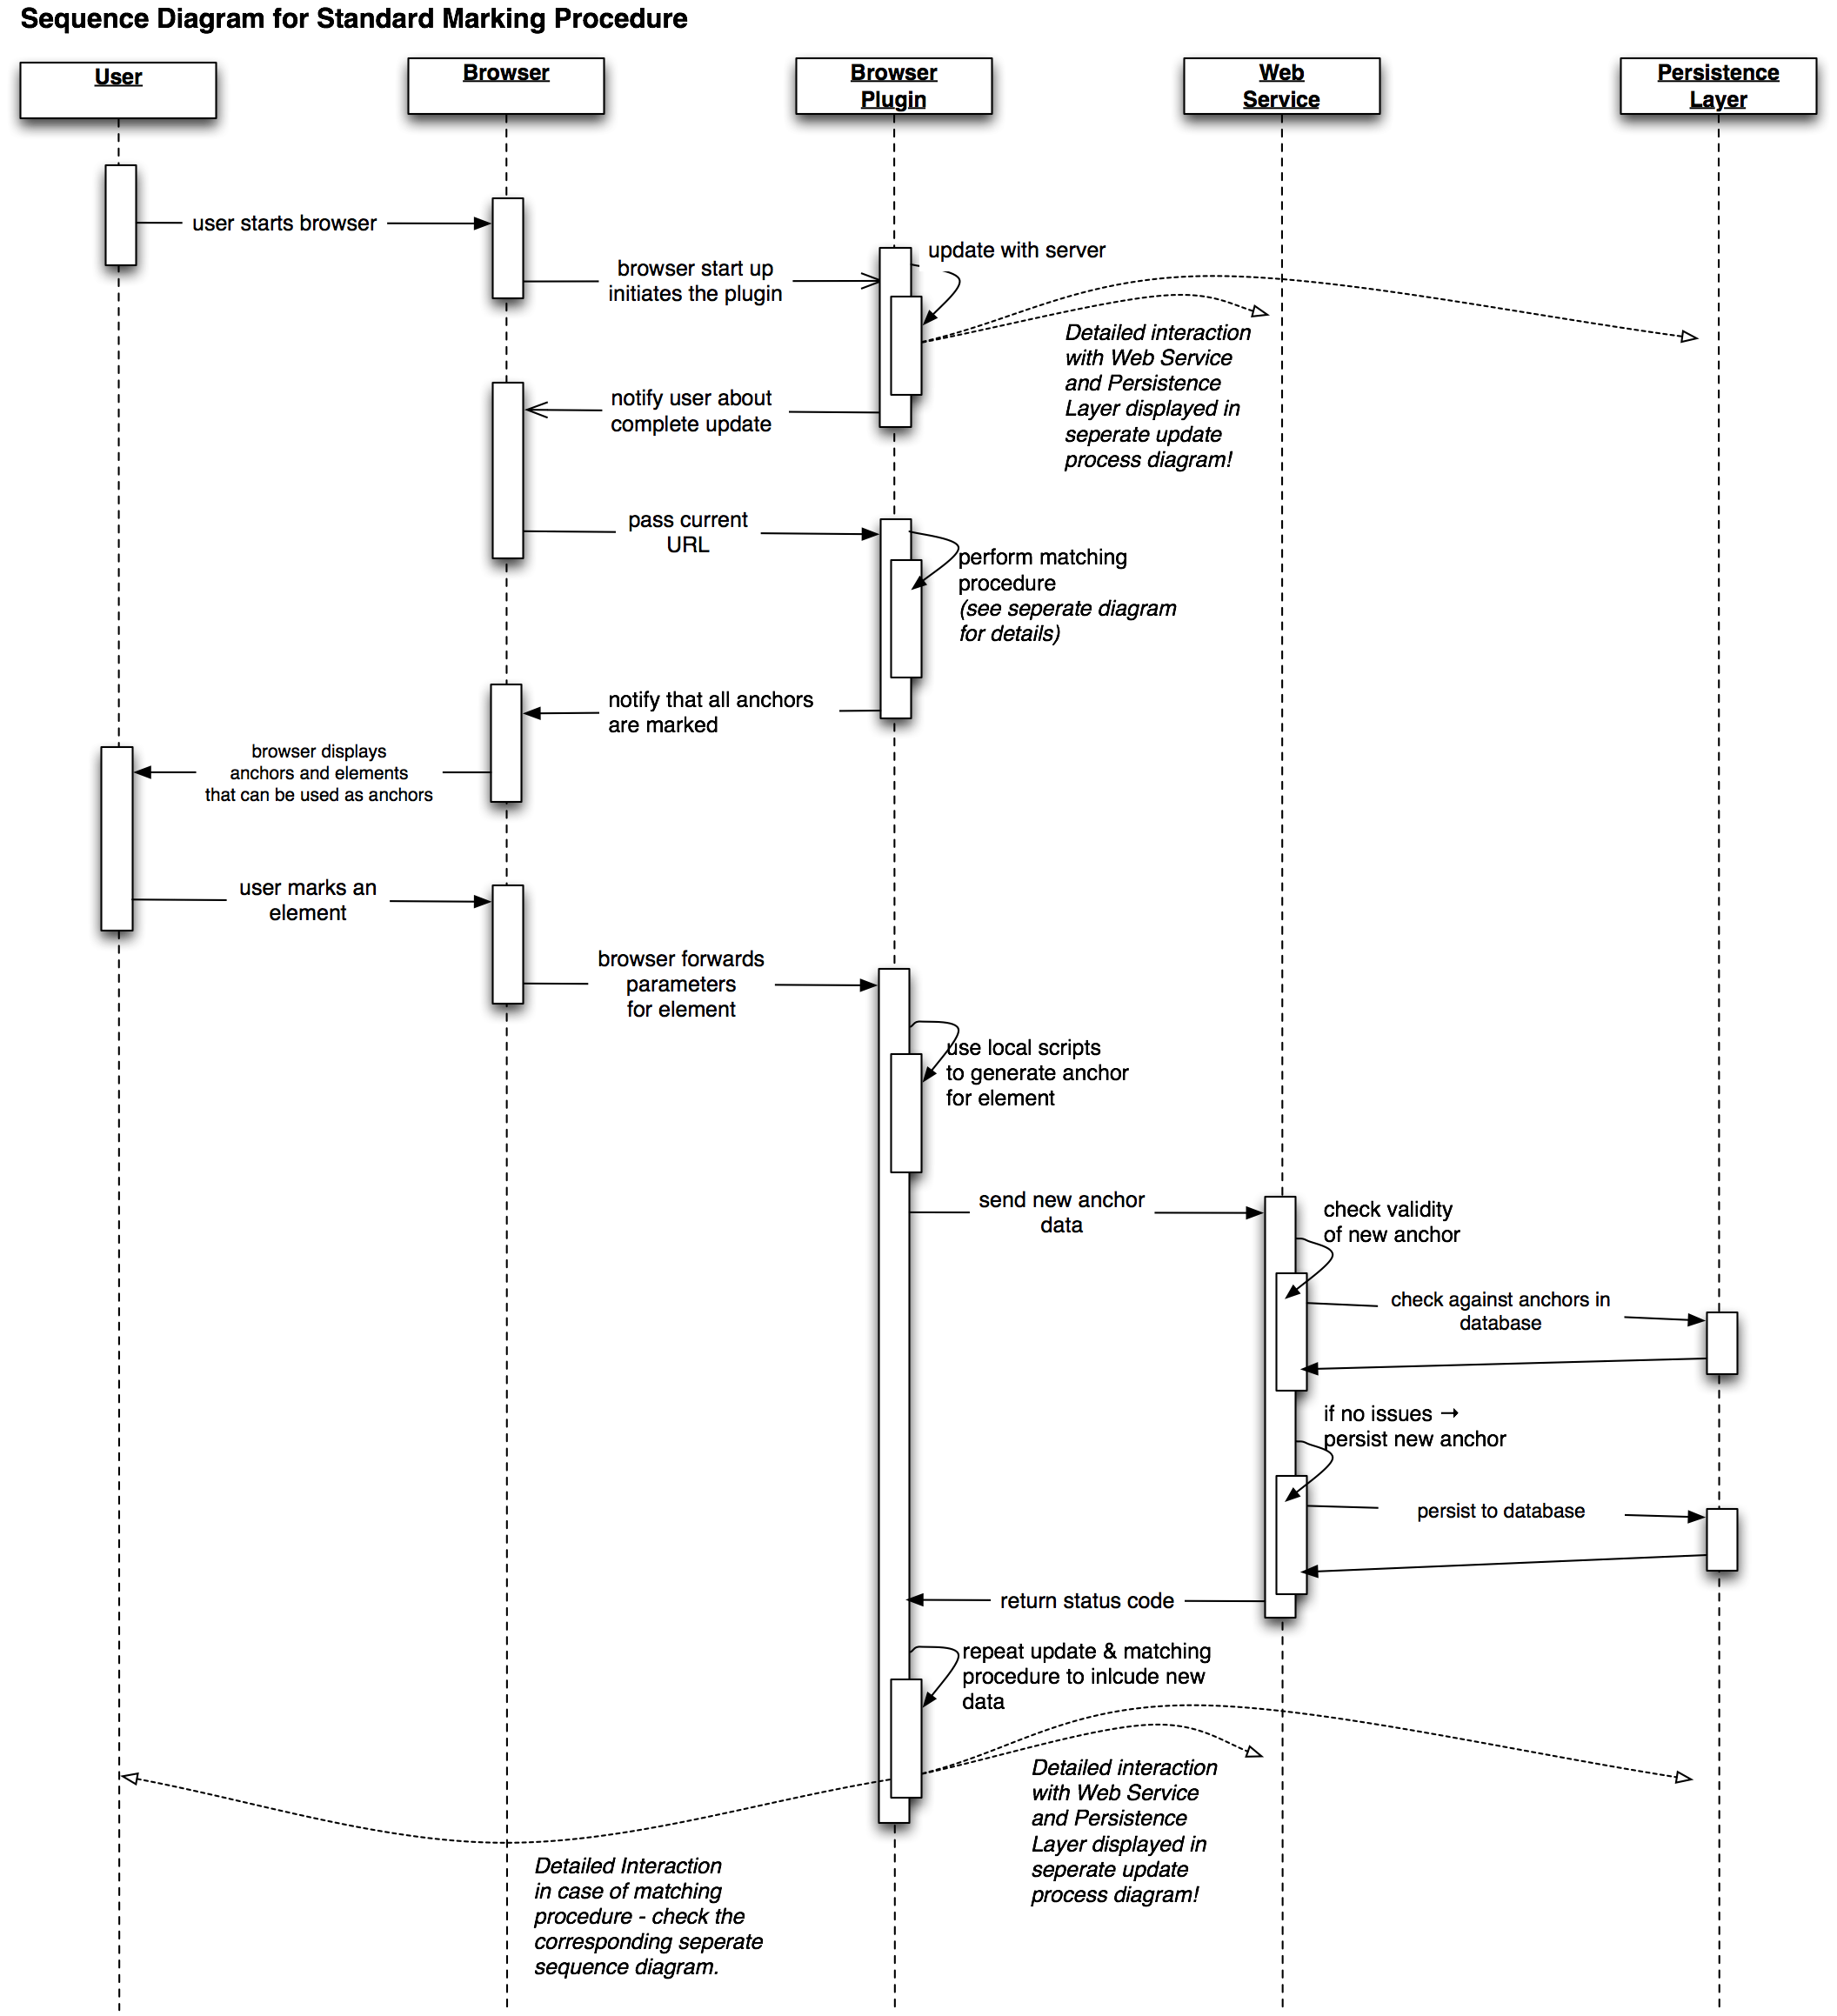
\includegraphics[width=13cm]{images/sequence-marking-process.png}
		\caption{Sequence diagram for standard marking procedure}
		\label{sequence-marking-process}
\end{figure} 

Finally it is possible for Alice to use the comment box. This step is very simple. As we already mentioned the comment box is an external service that is only injected by a link into our system. Therefore Alice can add a comment without any consequences to our system at all.

Now it is Bobs turn. This process is quite similar and partially redundant to what happened when Alice created the anchor. For that reason we will not got into detail like we did for the first step.

Bob opens the Google Calendar website, which triggers the update and matching procedure for this URL. Since there is an existing anchor now - Bob's plugin receives the data for displaying the comment box entered by Alice. 

The last two steps are getting more interesting again. We basically simulate a evolution of a website that destroys our anchor mechanism. That can happen very easily depending on the type of script we are using or how fast the webpage evolves, but this issue will be discussed more deeply in the coming section (\refname{sowe-assessment} \ref{sowe-assessment}). What we do is to modify the element identifier directly in the database. This way it becomes impossible to match this anchor for the given URL. 

So Alice visits her calendar to check whether Bob has answered her question. Again an update and matching procedure is started. The update will work seamlessly but an error occurs while the matching progresses. The plugin runs the script to determine the element that belongs to the element id - but with no success. 

For that case the plugin enables Alice to relink the content to the correct element or as in this case - appointment. The plugin performs the two following steps:
\begin{enumerate}
	\item Create a new anchor element, that is basically a copy to the old one but with a correct element-id. This step is identical to the above described procedure when Alice weaved the comment box into an appointment the first time. 
	\item  Additionally to the first step, we need to remove the broken anchor from the server. This is done by sending a remove Rest request to the server including the old element identifier. 
\end{enumerate} 
After those steps are finished, it is necessary to run the update and matching procedures again. Now Alice and Bob are able once again to use the comment box. 

Re-linking an anchor does not necessarly has to be due to an error or webpage evolution. For instance if Bob changed the time of the appointment - the anchor would not work either. In this case a re-link would solve the problem as well.

\newpage
\subsection{Social Weaver Scripts in Action}

\newpage
\subsection{Social Weaver Assessment}\label{sowe-assessment}
In the following we will analyse how good Social Weaver will work in several real scenario cases. Since it is developed as a proof-by-concept prototype, a general support for all web sites or web application was out of reach. Anyway the script support allows us to reach at least some flexibility. The testing range should cover static and more dynamic websites. Furthermore some freely available web applications will be tested. We will distinguish some criteria:
\begin{itemize}
	\item Level of Marking Support \\
	This criterion is the ability of the plugin to recognize elements in a web view. This means first of all that all relevant elements should be recognized. The best case would that elements like advertisements or scrolling bars would be left out. Still all buttons, form elements and similar elements would be spotted. This criterion is not purely objective since relevant elements may differ for each user.
	
	\item Level of Matching Support \\	
	Matching Support describes the ability of the plugin to find element that were previously marked. Even though this is at least as important as the Marking Support, there is no guarantee that matching will be handled equally well as marking. For instance if we match an element only by its path in the DOM tree; This path might be ambigious to another element. In this case our social element would be weaved into the wrong place. We consider this as the worst case even worse as if no element could have been matched.
 
	\item Level of Anchor Reliability \\
	Anchor Reliability can be seen as part of the matching criterion. But with reliability we refer to the time relevant aspect. With the evolution of a web page, our anchor information might become obsolete. The chance for this to happen is increasing with time. News pages are the best example for a very fast evolution. An anchor attached to an article on the frontpage would not last more than a couple of days. But even on such a dynamic web page there mostly are elements that are more reliable (e.g. the search column or navigation bars). 
	
	This criterion should evaluate how probably it is that anchors will outlast time. 
	
	\item Expense \\
	Expense in this context means how much effort has been used to give support for the tested environment. The extent of the script itself and an appraisal how tricky the construction of the script is, whether just standard procedure has been used or if it was necessary to insert some hacks. 
		
\end{itemize}